\documentclass{report}
\usepackage[T1]{fontenc} % Fontes T1
\usepackage[utf8]{inputenc} % Input UTF8
\usepackage[backend=biber, style=ieee]{biblatex} % para usar bibliografia
\usepackage{csquotes}
\usepackage[portuguese]{babel} %Usar língua portuguesa
\usepackage{blindtext} % Gerar texto automaticamente
\usepackage[printonlyused]{acronym}
\usepackage{hyperref} % para autoref
\usepackage{graphicx}
\usepackage[export]{adjustbox}
\usepackage{subfig}
\usepackage{afterpage}

\bibliography{bibliografia}


\begin{document}
%%
% Definições
%
\def\titulo{Computadores Quânticos}
\def\data{13 de Novembro de 2017}
\def\autores{Pedro Valente, Diogo Liebner}
\def\autorescontactos{(88858) pedro.valente@ua.pt, (89315) diogoliebner@ua.pt}
\def\versao{Versão 1}
\def\departamento{Departamento de Eletrónica, Telecomunicações e Informática}
\def\empresa{Universidade de Aveiro}
\def\logotipo{ua.pdf}
%
%%%%%% CAPA %%%%%%
%
\begin{titlepage}

\begin{center}
%
\vspace*{50mm}
%
{\Huge \titulo}\\ 
%
\vspace{10mm}
%
{\Large \empresa}\\
%
\vspace{10mm}
%
{\LARGE \autores}\\ 
%
\vspace{30mm}
%
\begin{figure}[h]
	\center
	\includegraphics{\logotipo}
\end{figure}
%
\vspace{30mm}
\end{center}
%
\begin{flushright}

\end{flushright}
\end{titlepage}

\null
\pagenumbering{gobble}
%% Título %%
\title{%
{\Huge\textbf{\titulo}}\\
{\Large \departamento\\ \empresa}
}
%
\author{%
    \autores \\
    \autorescontactos
}
%
\date{\data}
%
\maketitle

\clearpage
\null


\tableofcontents

 %\listoftables     % descomentar se necessário
 % \listoffigures    % descomentar se necessário


%%%%%% RESUMO %%%%%%
\chapter{Resumo}
\pagenumbering{arabic}
	O desenvolvimento dos computadores está limitada por duas barreiras intangíveis para o modelo atual: velocidade da luz no processamento da informação e a dimensão da ordem de grandeza atómica, no tamanho dos componentes num chip. Os \ac{cq} são o próximo passo para tentar atingir essas barreiras. A computação quântica  consegue resolver problemas exponencialmente mais rápido que os computadores de hoje em dia. Enquanto que os \ac{ct} usam transístores que trabalham com zero e uns, os \ac{cq} trabalham com todos os valores entre 0 e 1. Sendo assim tão rápidos, a segurança na Internet pode estar em risco pois conseguem resolver formulas de encriptação facilmente. Os \ac{cq} apresentam uma perspetiva positiva sobre o futuro.


%%%%%%%%%%%%%%%%%%%%%%%%%%%%
\clearpage
\null



\chapter{Introdução}
\label{chap.introducao}

	Com este trabalho temos o intuito de dar a conhecer uma nova tecnologia, uma nova espécie de computadores, os Computadores Quânticos.


	Estes computadores funcionam com bases de mecânica quântica e são extremamente mais rápidos que os computadores que usamos no dia a dia.


	Os computadores do dia a dia trabalham com bits, que podem assumir valores de 0 ou 1, contrariamente os \ac{cq} trabalham com qubits, que podem assumir valores de 0 e 1 ao mesmo tempo, assim como todos os valores entre estes. A vantagem que provém deste facto é que assim os \ac{cq} resolvem algoritmos de forma mais eficiente, e resolvem até problemas impossíveis para um computador regular.


	Mas os \ac{cq} não são só vantagens, estamos ainda muito longe de chegar ao ponto de os \ac{cq} substituírem os computadores regulares, apenas se conseguiu chegar a uma fração daquilo que se pensa que um computador quântico consiga fazer.

	Como motivação temos obviamente a esperança de um dia virmos a utilizar um destes computadores, se for de facto conseguido chegar-se a um computador quântico terminado, o ser humano dá um passo enorme na área tecnológica. Enquanto alunos do curso de Engenharia de \emph{Computadores} e Telemática (\ac{miect}) queremos obviamente ver novos e melhores computadores e os \ac{cq} são sem dúvida alguma o topo da escala.


	Este documento está dividido em onze capítulos.
	Depois desta introdução,no \autoref{chap.História} são apresentados alguns anos nos quais houve marcos históricos na vida dos \ac{cq}, este capítulo está dividido em sete secções. No \autoref{chap.Como funcionam ?} é explicado como funcionam os \ac{cq}.
	No capítulo seguinte \autoref{Modelos}, dividido em quatro secções são apresentados alguns modelos de \ac{cq}.
	No capítulo \autoref{chap.Implementações Físicas de Computadores Quânticos}, dividido também em quatro secções são referidos alguns complementos  de fisíca na construção de \ac{cq}.
	No capítulo \autoref{chap.segurança} falamos de como a segurança dos nossos dados na web pode estar em perigo devido à facilidade com que os \ac{cq} conseguem desmantelar os nossos \ac{sc} atuais.
	No capítulo \autoref{chap.D-Wave} divido em duas secções, na primeira é falado um pouco sobre esta empresa e na segunda referimos alguma controvérsia que houve em torno da empresa no geral e na veracidade do seu trabalho.
	No capítulo \autoref{chap.comparação}  que está dividido em 3 secções comparamos um \ac{cq} a um \ac{ct}.
	Por fim temos o capítulo \autoref{chap.conclusao} que é a conclusão,o capítulo \autoref{agradecimentos} agradecemos a quem nos ajudou a fazer este trabalho, o capítulo \autoref{contribuição} onde referimos a contribuição de cada um dos dois autores deste trabalho, o capítulo \autoref{acrónimos} onde referimos cada acrónimo utilizado e para terminar o trabalho temos o capítulo \autoref{chap.Bibliografia} onde referimos os locais utilizados para recolha de informação para a realização do trabalho.

\chapter{História}
\label{chap.História}

\section{1981}


	Em 1981 o físico norte-americano Richard Feynman deu o primeiro passo ao aplicar mecânica quântica em em simples atividades computacionais.

	O raciocínio de Feynman surgiu quando este verificou que um computador normal leva demasiado tempo para simular um simples exercício de física quântica, mas que por outro lado, sistemas quânticos de grande simplicidade conseguiam resolver grandes quantidades de cálculos em pouco tempo.

	Feynman pensou então que esta capacidade poderia ser muito útil.

\section{1985}


	Em 1985 o físico israelita David Deutsch descreveu o primeiro computador quântico universal.

	David Deutsch concluiu que  um computador quântico universal é capaz de simular o funcionamento de outro computador quântico de maior complexidade.

	Isto criou expectativas de que um simples dispositivo fosse capaz de resolver grandes quantidades de cálculos e/ou algoritmos quânticos.

\section{1994}
\label{subsec.chap}

	Em 1994 o matemático norte-americano Peter Shor descobriu um algoritmo que permite a um computador quântico realizar a fatorização de números inteiros muito grandes. Este algoritmo de Shor será de extremo interesse no contexto dos computadores quânticos pois conseguiria desmantelar muitos dos \ac{sc} atuais.

\newpage

\section{1996}

	Em 1996 o indiano-americano Lov Grover descobriu o algoritmo utilizado para a pesquisa em bases de dados quânticas.

	Também neste ano, é feita uma proposta para o primeiro esquema para a correção de erros quânticos.

	Assim o computador passa a conseguir encontrar e corrigir erros, mas esta proposta trazia consigo o problema de que o computador apesar de conseguir corrigir alguns dos erros este não os consegue corrigir durante o próprio processo de correção.

	Já foram propostas algumas resoluções para este problema mas a pesquisa mantém-se.

\section{1999}

	Alguns engenheiros do \ac{mit}  construiram os primeiros \ac{cq} no ano de 1999.

\section{2007}

	Em 2007 a  empresa canadiana D-Wave afirma ter desenvolvido um computador chamado Orion, que era um híbrido(tanto era quântico, como era um computador regular).

	Se tal for confirmado, o Orion será então o primeiro computador quântico capaz de resolver tarefas práticas, seria capaz de resolver um jogo de \verb/Sudoku/ ou até encontrar alternativas para medicamentos usados na indústria farmacêutica.

	Apesar disto o Orion não tinha o que era preciso para ter aplicação comercial.

	Mas a D-Wave afirma que num futuro próximo irá conseguir atingir um computador com 1 quiloqubit. Algo que a comunidade científica recebeu com algum ceticismo pois a empresa não entrou em detalhes sobre o processador deste computador.

	\begin{figure}[!h]
		\centering
		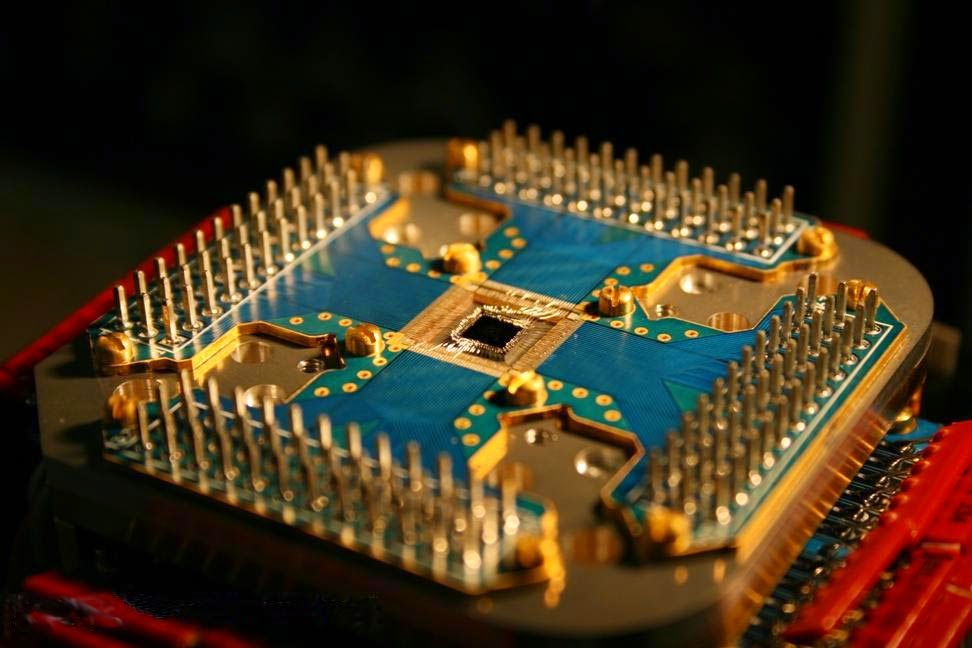
\includegraphics[scale=0.17]{Orion.jpg}
		\caption{Computador Quântico Orion}
		\label{Orion}
	\end{figure}

\section{2017}

	Em 2017 a empresa D-Wave lançou então comercialmente o 2000Q, um computador quântico com 2000 qubits, lançado a um preço de 15 milhões de dólares, falamos mais sobre este computador mais à frente no trabalho.

\clearpage
\null
\chapter{Como funcionam os Computadores Quânticos ?}
\label{chap.Como funcionam ?}

	Um \ac{cq} pode conter 16 valores analógicos aos pares para formar 8 números complexos, ou seja, poderia conter a seguinte tabela:

\begin{center}
\begin{table}
\begin{tabular}{|c |c |c|}
\hline
 Estado & Amplitude & Probabilidade \\ 
 \hline
  * & (a+ib) & $(a^2 + b^2 )$ \\
 \hline  
 000 & 0.37+i0.04 & 0.14 \\
 \hline
 001 & 0.11+i0.18 & 0.04 \\
 \hline
 010 & 0.09+i0.31 & 0.10 \\
 \hline
 011 & 0.30+i0.30 & 0.18 \\
 \hline
 100 & 0.35+i0.43 & 0.31 \\
 \hline
 101 & 0.40+i0.01 & 0.16 \\
 \hline
 110 & 0.09+i0.12 & 0.02 \\
 \hline
 111 & 0.15+i0.16 & 0.05 \\
 \hline
\end{tabular}
\centering
\caption{Estado, Amplitude e Probabilidade dos qubits}
\end{table}
\end{center}



	Esta tabela teria $2^n$ linhas se existissem n qubits.
 \verb|Curiosidade:| Para um n na ordem das centenas, tal seria mais linhas do que os átomos que são conhecidos no universo.
 
	Na primeira coluna é mostrado todos os estados possíveis para três bits, um computador quântico pode assumir 8 estados em simultâneo.

	Na segunda coluna é representada a amplitude para cada um dos oito estados.

	Todos os oito números complexos são uma representação dos \ac{cq} 
num momento exato.

	 Durante a computação, estes 8 números irão modificar e interagir uns com os outros. Neste sentido, um computador quântico de 3 qubits tem muito mais memória do que um computador clássico de 3 bits.
 
	Na terceira coluna da tabela é calculada a probabilidade de cada linha possível. 			Cada uma destas probabilidades é encontrada através do cálculo do módulo do quadrado do número complexo.
	Todas as probabilidades somadas irão resultar em 1.

	Para uma máquina que esteja finalizada, a operação é realizada ativando um pequeno pulso de radiação no local onde estão as moléculas, para diferentes tipos de pulsos temos resultados diferentes(matrizes diferentes).

	O algoritmo chave para um computador quântico consiste na escolha dos pulsos a usar e na ordem em que devem ser usados, esta ordem é normalmente escolhida de forma a que todas as probabilidades tendam para 0 exceto uma, probabilidade esta que será aquela que corresponde à resposta correta. Sendo assim, depois de ter todos os cálculos feitos, esta resposta é a que terá a maior probabilidade de ser escolhida e retornada.

	Mas mesmo assim, há vários modelos de computadores quânticos, seram então referidos alguns destes modelos no próximo capítulo.

\chapter{Modelos de Computadores Quânticos}
\label{Modelos}

\section{Quantum annealing}
\label{Quantum-annealing}

	\emph{Quantum annealing} é um processo usado pela empresa D-Wave (\ref{D-Wave}), que tem como objetivo procurar soluções para resolver problemas.

	\emph{Quantum annealing} recorre  às tendências naturais de sistemas quânticos para encontrar estados de baixa energia.

	 Se a optimização de um problema for análoga à paisagem de montanhas e vales e  se cada coordenada representa uma solução possível e a sua elevação representa a energia, a melhor solução é a que contém a menor energia, que é correspondente ao ponto mais fundo do vale, naquela paisagem.
 
	É então assim que \emph{Quantum annealing} funciona.

	Este tema é um pouco abordado mais à frente na secção \ref{controvérsia}.

\section{Modelo de CQ topológico}
\label{Topológico}
	Um \ac{cq} topológico é por agora, nada mais que um conceito teórico, visto que este se baseia apenas em quasipartículas de duas dimensões conhecidas por \verb|anyons|.

	A existência destas \verb|anyons| foi comprovada por um grupo de cientistas de "Stony Brook University" no ano de 2005. Foi comprovado que estas não eram simplesmente uma construção matemática.

	Infelizmente esta experiência permanece sem ser aceite por completo pela comunidade científica.

	O modelo topológico utiliza as \verb|anyons| para formar tranças em três dimensões no espaço-tempo, tranças estas que formam por sua vez as portas lógicas do computador, tendo a vantagem de possuirem uma maior resistência ao ruído externo.

\section{CQ adiabático}
\label{adiabático}

	Este modelo de computação quântica é baseado num teorema chamado teorema adiabático.

	\textbf{Teorema adiabático:} Se um sistema quântico for alterado devagar o suficiente, este irá ter tempo de se poder adaptar, ou seja, se o sistema se encontrava inicialmente no seu estado próprio do Hamiltoniano inicial, irá também terminar no seu estado próprio correspondente do Hamiltoniano final.

	Sendo assim, num \ac{cq} de modelo adiabático, encontra-se um Hamiltoniano complexo cujo estado fundamental irá descrever a solução do problema em questão. Depois disso um Hamiltoniano simples é iniciado no seu estado fundamental, e através do método adiabático, o referido Hamiltoniano simples dá lugar a um complexo, no qual o istema continua no estado fundamental, sendo este último a resposta ao problema que lhe foi proposto.

\section{Modelo do Circuito Quântico}

	Este modelo, à semelhança de um \ac{ct} dá uso a portas lógicas, só que este usa portas lógicas quânticas em vez de regulares.

	Exemplo de portas lógicas : AND, OR, NOT, NAND, etc...

	No entado as portas lógicas quânticas têm obrigatoriamente que ser reversíveis, ou seja, a informação que está na saída da porta, tem que conter uma operação inversa que permita, por sua vez, obter uma entrada.

	De seguida vamos mostrar dois exemplos de portas lógicas quânticas:

\begin{itemize}
  \item Porta \textbf{Hadamard} que atua num único qubit
  
  \begin{figure}[!h]
	\centering
	\subfloat[Matriz Hadamard]{
	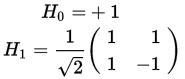
\includegraphics[scale=0.5]{matrizhadamart.png}
	\label{Matriz Hadamart}
	}
	\qquad
	\subfloat[Porta Hadamard]{
	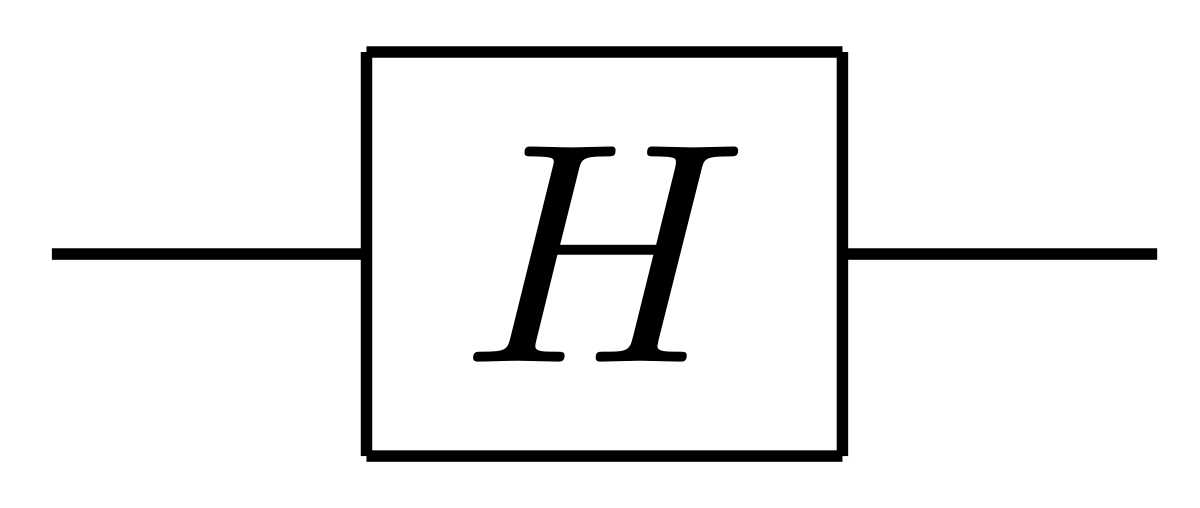
\includegraphics[scale=.08]{portahadamart.png}
	\label{Porta Hadamart}
	} 
\end{figure}
  
  
  \item Porta \textbf{CNOT}	(\textit{Controlled NOT gate}) que atua em dois ou mais qubits
  
   \begin{figure}[!h]
	\centering
	\subfloat[Matriz CNOT]{
	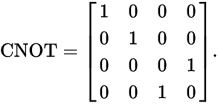
\includegraphics[scale=0.5]{matrizcnot.png}
	\label{Matriz CNOT}
	}
	\qquad
	\subfloat[CNOT gate]{
	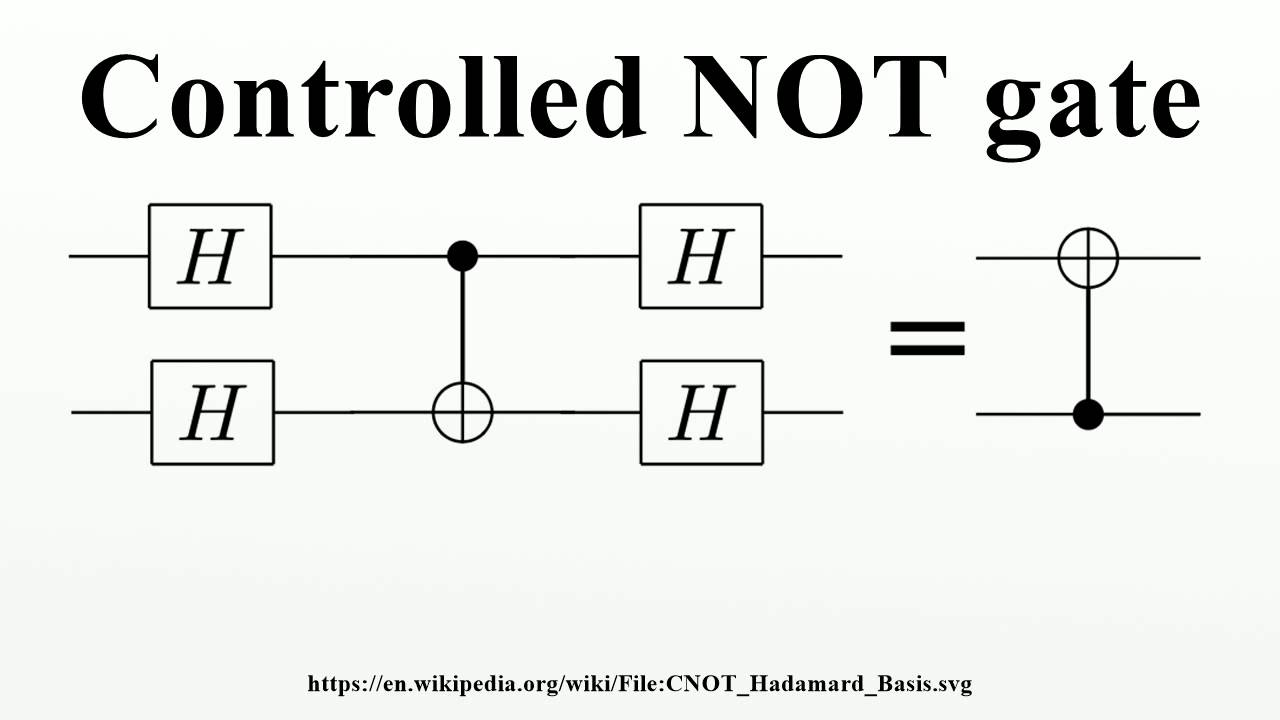
\includegraphics[scale=.08]{cnot.jpg}
	\label{CNOT}
	} 
\end{figure}
\end{itemize}


\chapter{Implementações Físicas de Computadores Quânticos}
\label{chap.Implementações Físicas de Computadores Quânticos}

\section{CQ à base de supercondutores}
	Nos dias que correm muitos dos \ac{cq} que são produzidos em laboratório são feitos à base de supercondutores.

	Supercondutividade é o fenómeno que acontece quando os cetos materiais se encontram a uma temperatura menor da sua temperatura crítica, fazendo com que estes materiais acabem por não ter qualquer resistência elétrica.


	A supercondutividade é então utilizada na construção de alguns aparelhos tais como a junção de Josephson (Josephson junction) e os SQUID (superconducting quantum interference device) ou dispositivos supercondutores de interface quântica, que serão então depois usados na construção de computadores quânticos deste tipo.

\begin{figure}[!h]
	\centering
	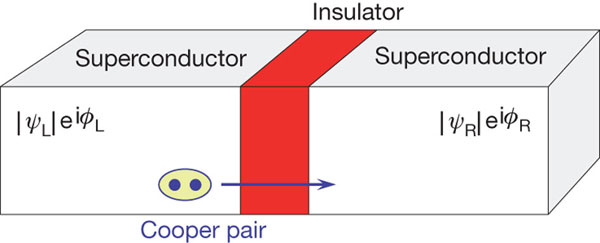
\includegraphics[scale=0.5]{Josephson-junction.jpg}
	\caption{Junção de Josephson}
	\label{Junção de Josephson}
\end{figure}

\newpage

	A junção de Josephson  é composta por dois supercondutores com um isolante extremamente fino no meio, é graças a estes supercondutores que a corrente é capaz de fluir indefinidamente sem a aplicação de qualquer tensão e, pode atravessar a barreira isolante devido ao efeito de túnel quântico.

	Por outro lado, os SQUID são feitos a partir de várias junções de Josephson, são bastante pequenos e têm uma grande sensibilidade a campos magnéticos.

	\ac{cq} que utilizam supercondutores são obrigados a estar a temperaturas de poucos Kelvin, o que por sua vez requer que sejam utilizados sistemas de refrigeração específicos.



\section{CQ de iões presos}

	Os \ac{cq} de iões presos são considerados os mais fortes candidatos no que toca à cosntrução de um computador quântico universal. 

	Os iões (átomos com carga) são chamados presos porque ficam, exatamente como o nome indica, presos num espaço vazio que utiliza campos eletromagnéticos.
Como exercer forças elétricas em toda e qualquer  direção do espaço não é possível, pois estas iriam anular-se umas às outras, é aplicada uma força elétrica com um comportamento  oscilatório a uma elevada frequência, de forma a prender o ião no centro através da inércia.


	Seguidamente, é dado uso a lasers para que se possam realizar as operações que sejam necessárias  nos iões, os qubits.

\newpage

\section{CQ à base de uma rede ótica}

	Uma rede ótica, ou \verb|Optical lattice|, é constituída pelo cruzamento de feixes de laser, criando uma polarização espacial, criando também desta forma poços de potencial.


	De seguida  é efetuado o arrefecimento dos átomos de forma a serem condicionados no seu ponto mínimo de potencial.

	Serão também utilizados átomos neutros em vez de iões, para prevenir interações indesejadas entres estes e as forças eletromagnéticas do ambiente em seu redor, isto devido à sua carga.

	Por fim, é dado uso a um segundo grupo de lasers para que estes possam controlar o estado dos átomos, os qubits, de forma que estes possam executar as operações dos \ac{cq}.

\begin{figure}[!h]
	\centering
	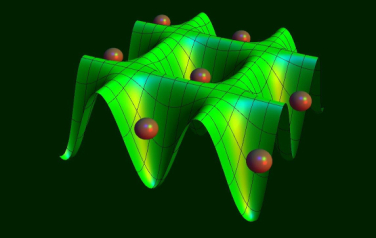
\includegraphics[scale=0.5]{redeotica.jpg}
	\caption{Rede ótica, a verde os poços de potencial e a castanho, os átomos}
	\label{Rede otica}
\end{figure}

\clearpage

\section{CQ à base de diamante}

	Os \ac{cq} à base de diamante, fazem uso de uma propriedade dos diamantes denominada \verb|Nitrogen-vacancy center|, que é um ponto defeituoso dos diamantes, no qual o átomo de carbono foi substituído por um átomo de nitrogénio e por um eletrão.

	Numa experiência realizada em Abril de 2012, o átomo de nitrogénio foi utilizado como qubit e o eletrão foi utilizado como segundo qubit.

	O estado dos qubits pode ser controlado pode ser monitorizado utilizando impulsos de microondas. O facto de este se encontrar dentro do diamante, concede ao diamante uma proteção no que toca a ruídos externos que iriam causar decoerência quântica.


\begin{figure}[!h]
	\centering
	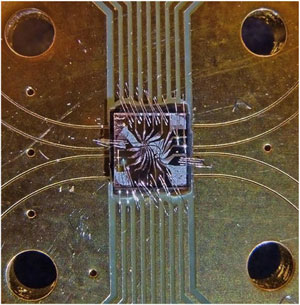
\includegraphics[scale=0.5]{diamante.jpg}
	\caption{CQ à base de diamante}
	\label{diamante}
\end{figure}


\chapter{Segurança}
\label{chap.segurança}


	Os \ac{cq} são uma ameaça enorme à segurança na Internet. A partir do momento que um deles é ligado a um servidor com acesso a todos os dados do mundo, o \ac{cq} consegue aceder a todas essas informações encriptadas.
	
	Hoje em dia a Internet usa dois métodos de encriptar, criptografia de chave simétrica e criptografia de chave assimétrica(ou chave pública).
	
	Criptografia de chave simétrica é mais rápida e mais segura que a sua contraparte mas requer que a chave de encriptação seja conhecida entre os dois locutores. Estes guardam a chave num lugar que os dois consideram seguro. Um método específico de cifra de chave simétrica é a troca de chave do Diffie-Hellman. Foi desenvolvida por Whitfield Diffie e Martin Hellman e publicado em 1976.
	
	Criptografia de chave assimétrica é a mais usada entre as duas. Neste caso todos os utilizadores na rede têm acesso à chave pública de um computador para poder enviar informação porém só esse computador pode aceder a essa informação que lhe foi enviada com a sua chave privada. As chaves atualmente são equações matemáticas muito complexas e devem ser quase impossíveis de resolver para computadores tradicionais. O algoritmo de criptografia mais bem sucedida no sistema de chaves assimétricas é a RSA.
	
	\newpage
	
	 O seu nome tem origem em três professores do \ac{mit}, Ronald \textbf{R}ivest,  Adi \textbf{S}hamir e Leonard \textbf{A}ldeman, fundadores da atual empresa \textbf{RSA Data Security, Inc.}

\begin{figure}[!h]
	\centering
	\subfloat[Algoritmo Troca de Chaves]{
	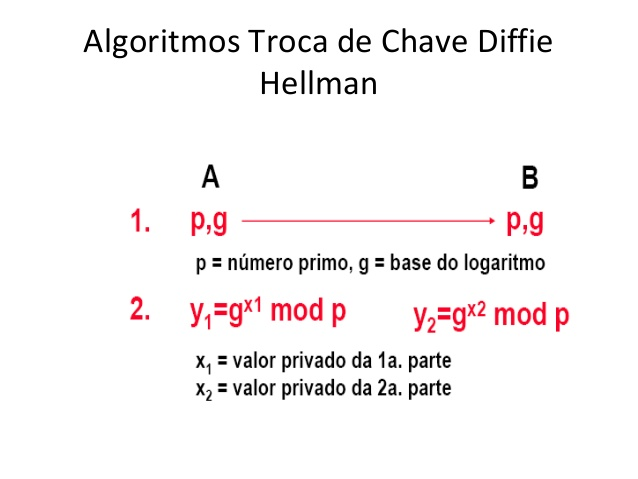
\includegraphics[scale=0.20]{trocadechaves.jpg}
	\label{Algoritmo Troca de Chaves}
	}
	\qquad
	\subfloat[Criptografia de RSA]{
	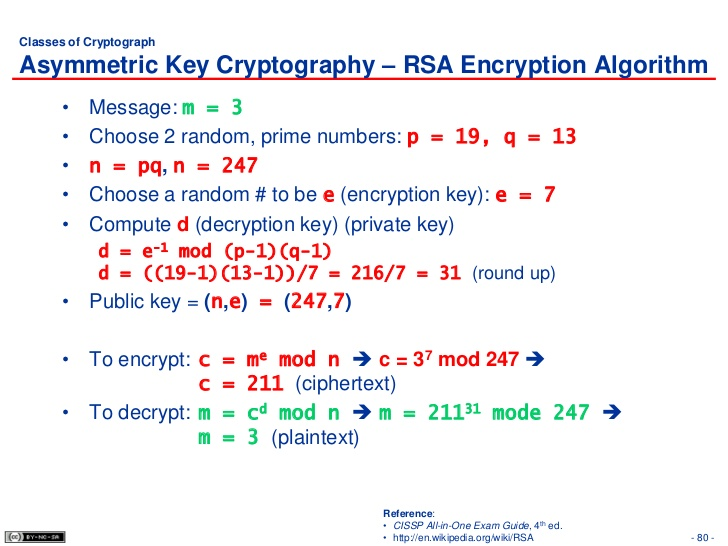
\includegraphics[scale=.2]{RSA_criptografia.jpg}
	\label{Criptografia de RSA}
	} 
\end{figure}	

	Tendo em conta a potência dos \ac{cq}, as chaves públicas e privadas podem vir a ser completamente inúteis. Na contemporaneidade os \ac{cq} ainda não conseguem fazer nada de importante nesta área, mas é razoável assumir que estarão após o ano 2025. 
	

	
	Diante disso Tanja Lange, professora de Criptologia na Universidade de Tecnologia em Eindhoven, conduz a investigação de Criptografia \emph{Post-Quantum}, ou \emph{PQCrypto}, que combina o poder intelectual de 11 universidades diferentes e empresas para tentar encontrar uma nova maneira de encriptar informação. Esta investigação apenas começou em 2015 e Lange avisa que pode demorar até 20 anos para conseguir encontrar uma nova maneira de cifrar mensagens.
	
\begin{figure}[!h]
	\centering
	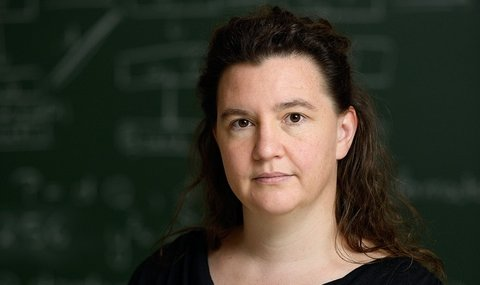
\includegraphics[scale=0.3]{Tanja_Lange.jpg} 
	\caption{Tanja Lange}
	\label{Lange}
\end{figure}
	

\chapter{D-Wave}
\label{chap.D-Wave}
	\begin{figure}[!h]
		\centering
		
\includegraphics[scale=0.5]{Logo_D-Wave.jpg} 
		\caption{Logo da empresa D-Wave}
		\label{D-Wave}
		
	\end{figure}		
	

\section{Sobre}
	D-Wave é a empresa principal no que toca ao desenvolvimento de computação quântica comercial. Foi fundada no ano 1999 no Canadá, na costa Oeste, por Geordie Rose e Haig Farris(Mentor académico do Geordie Rose).
	
	No ano de 2011 anunciaram que iam lançar para o mercado comercial o primeiro computador quântico do mundo, o \textbf{D-Wave One}. Custa 10,000,000\$ e continha um processador de 128 qubits, no entanto só podia funcionar em conjunto com \ac{ct} e para entrar no estado quântico tinha que ser arrefecido por hélio até 0.02K de temperatura.


	\begin{figure}[!h]
		\centering
		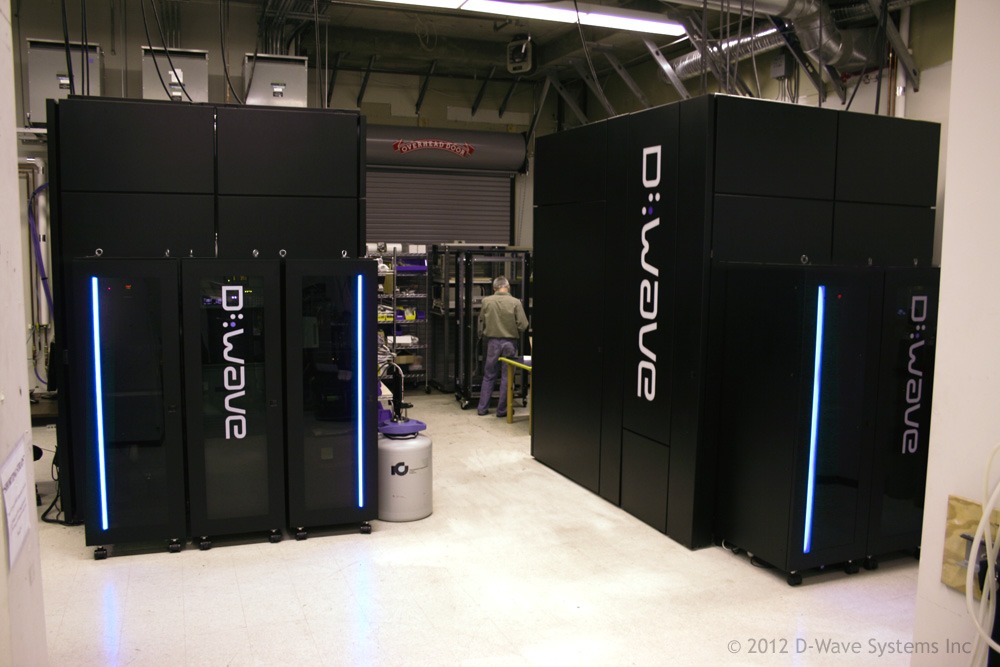
\includegraphics[scale=0.43]{dwave_ones_in_the_lab_large.jpg} 
		\caption{Foto de dois computadores \textbf{D-Wave One}}
		\label{D-Wave}
	\end{figure}	
		
	\newpage
	
	Em 2013 lançaram o segundo modelo comercial deles,\textbf{D-Wave Two} que continha 512 qubits.

	O computador mais recente no entanto é o \textbf{D-Wave 2000Q}, e tal como o nome indica, tem um processador de 2000 qubits. Na data de escrita é o \ac{cq} mais avançado à face da terra. Este modelo tem pouco acima de 3 metros de altura por causa do 'frigorífico' extremo que baixa a temperatura até os 0.0015K, 180 vezes mais frio que o espaço interstelar. O ambiente de processamento também é único visto que existe pressão 10 mil milhões de vezes menor que a pressão atmosférica. Consome 25 kW de energia e esse número provavelmente não aumentar com gerações sucessivas segundo a D-Wave.


	\begin{figure}[!h]
		\centering
		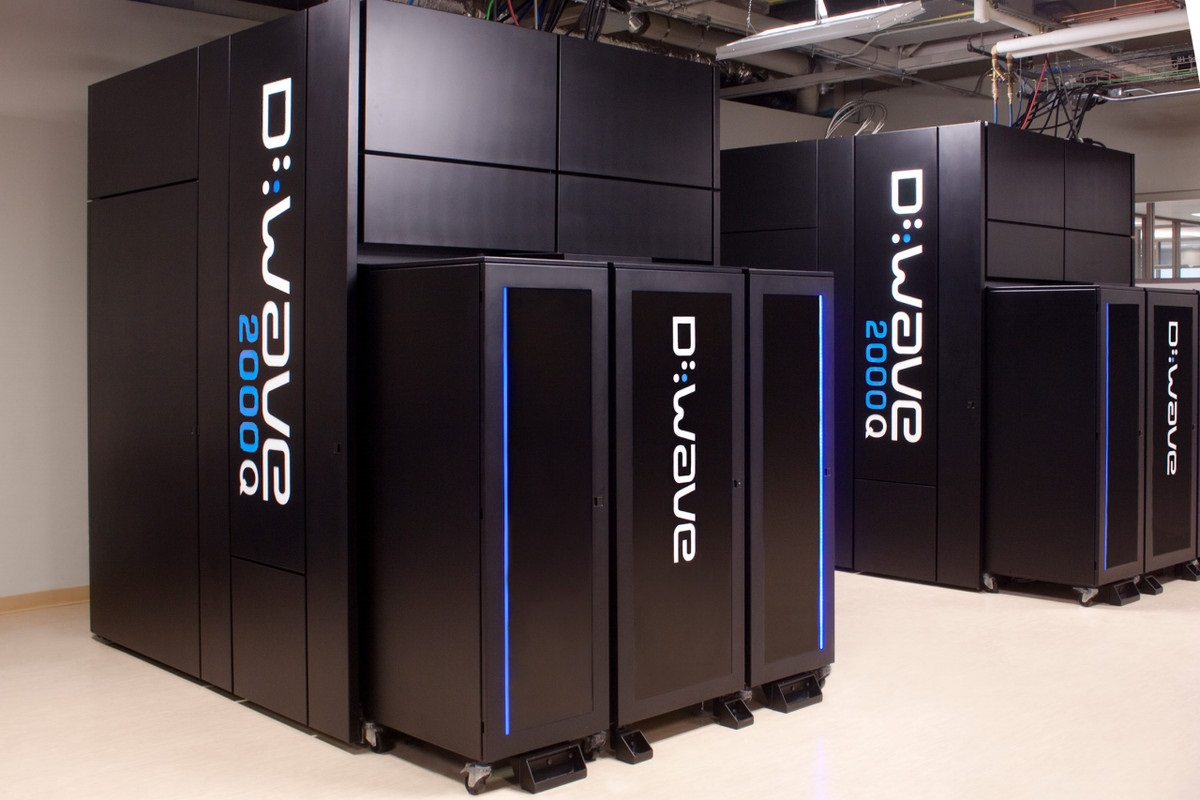
\includegraphics[scale=0.18]{D-Wave-2000Q.jpg} 
		\caption{Foto de dois computadores \textbf{D-Wave 2000Q}}
		\label{D-Wave}		
	\end{figure} 

\section{Controvérsia}
\label{controvérsia}

	Todavia não existem produtos sem alguma polémica. Mesmo que o último modelo da D-Wave tenha um processador de 2000 qubits, 1000 qubits mais que a versão anterior, ninguém o está a comparar. Independentemente da confiança da D-Wave, cientistas e académicos dizem que a empresa nunca provou as vantagens em relação a \ac{ct}. E ainda pior, se continuarem a usar a mesma metodologia, nunca vão.
	
	O diretor de desenvolvimento de negócios da empresa e um ex cientista de computação quântica Colin Williams,declara \emph{quantum annealing} é a melhor maneira de fazer um computador quântico. Williams afirma que o método tem imensas vantagens sobre os outros esquemas. Existe interesse da parte da Microsoft em relação à computação quântica topológica, mas Williams defende que é demasiado teórica e muito difícil de trabalhar com essa tecnologia.

	Mais explicações sobre \emph{quantum annealing} na secção \ref{Quantum-annealing}.
		
	Contudo, um estudo publicado na revista \textit{Science} em 2014 demonstrou que tarefas completas num computador da D-Wave não foram mais rápidas que as tarefas num \ac{ct}. Os investigadores estavam à procura de um \emph{quantum speedup}, a vantagem principal dos \ac{cq} que defende que quanto mais cálculos se atira à maquina, maior se vê a diferença entre computadores quânticos e tradicionais. 
	
\newpage
	
	O artigo no \textit{Science} não exclui a possibilidade de existir esse \emph{quantum speedup} mas certamente não encontraram evidência da existência dela.
	
	Matthias Troyer, coautor da publicação na revista \textit{Science} em 2014,  indica que a arquitetura implementada no D-Wave, a computação pode ser imitada eficientemente num \ac{ct}. Segundo Troyer simplesmente dobrando o numero de qubits nos chips não vai ajudar D-Wave ultrapassar este problema, visto que não encontraram nenhuma prova do \emph{quantum speedup}.

\begin{figure}[!h]
		\centering
		\subfloat[Colin Williams]{
		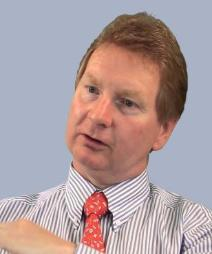
\includegraphics[height=4cm]{Colin_Williams.jpg}
		\label{Colin Williams}
		}
		\qquad
		\subfloat[Matthias Troyer]{
		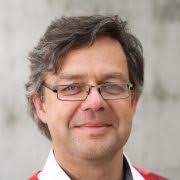
\includegraphics[height=4cm]{Matthias_Troyer.jpg}
		\label{Matthias Troyer}  
		}
\end{figure} 


 
\newpage

\null
\chapter{Comparação}
\label{chap.comparação}
\section{Consumo de energia}
	Tal como referido no capítulo anterior, o último modelo da linha de computadores da D-Wave gasta apenas 25 kW de energia, da qual maior parte é usada para manter o sistema numa temperatura que o mantém funcional. Os supercomputadores tradicionais no entanto podem chegar a um consumo de energia de 4.04 MW. Deste modo os \ac{ct} consomem 161 vezes mais energia que os \ac{cq}.
	

\section{Velocidade de processamento}
	A vantagem dos \ac{cq} nesta área em relação aos \ac{ct} é que (supostamente) possuem o que se designa \emph{quantum speedup}. Isto ajuda imenso na resolução de problemas matemáticos de uma forma exponencial. O \emph{quantum speedup} é tão potente que pode resolver problemas em poucas horas que pode deixar um computador normal a trabalhar durante anos
	
	Sem dúvida alguma, uma das competências mais esperadas de um \ac{cq} é o facto de este poder fazer a fatorização de grandes números, como já referido anteriormente na secção \ref{subsec.chap} . Por exemplo, se um número tiver um número n de bits, então um computador com cerca de 2n qubits conseguirá encontrar os seus fatores. 
	
\newpage
	
	Atualmente é sabido que a vantagem dos \ac{cq} só é notada em três problemas: fatorização, logaritmo e simulações de física quântica.
	
\begin{figure}[!h]
	\centering
	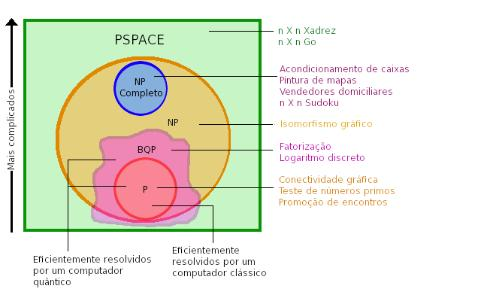
\includegraphics[scale=0.3]{potencial.jpg} 
	\caption{Fatorização e Logaritmo Discreto}
	\label{potencial}
		
\end{figure}	

	No ano 2017 os \ac{cq} da D-Wave já conseguiram contribuir bastante para algumas investigações. Em outubro o algoritmo quântico da D-Wave ajudou a compreender um bocado melhor a partícula \emph{Higgs Boson} e em agosto resolveu o mistério de como certas proteínas dobram.
		
	Um \ac{cq} baseado em protões e neutrões de uma molécula, irá ser de tão pequenas dimensões que o olho humano não o conseguirá ver, mas por outro lado conseguiria fatorizar números inteiros com milhares e milhares de bits. Enquanto que um \ac{ct}, para conseguir realizar este tipo de contas antes de o sol desaparecer, teria que ser do tamanho de todo o universo, o que não é de todo prático.

\newpage

\section{Uso pessoal}
	Uma das desvantagens dos \ac{cq} é que provavelmente não vão estar disponíveis para uso pessoal no futuro próximo. Precisam de demasiado espaço só para poder manter o ambiente de processamento estável, e frio que chegue a fim de haver o tal estado quântico no processador (D-Wave 2000Q tem 3 metros de altura)

\clearpage
\null
\chapter{Conclusão}
\label{chap.conclusao}

	A computação quântica é a ferramenta que irá ajudar imensos investigadores nos seus estudos em que os \ac{ct} não têm capacidade de processamento que chegue. Com numerosas empresas como a NASA, Microsoft, Google, etc. interessados nesta área, o objetivo para atingir é substituir completamente os supercomputadores atuais. Este processo de substituição ainda está na sua infância pelo que os ainda não são completamente compreendidas todas as possibilidades de criação de um processador quântico, mas é previsto que esta substituição vá acontecer por volta do ano 2025 segundo alguns cientistas.


%%%%%% Agradecimentos %%%%%%

\clearpage
\null
\chapter{Agradecimentos}
\label{agradecimentos}
	No âmbito da disciplina de Laboratório de Informática, agradecemos aos alunos de outras matriculas que nos ajudaram a trabalhar no GIT e no \LaTeX . Agradecemos também o nosso professor de LABI Óscar Pereira pela ajuda fornecida durante as aulas. E um último agradecimentos a uns colegas da nossa matricula que nos ajudaram no GIT.

\clearpage
\null
\chapter{Contribuições dos autores}
\label{contribuição}
	O autor \ac{pvm} fez a introdução, o funcionamento dos computadores quânticos, os modelos dos computadores quânticos e as implementações físicas.
O autor \ac{dl} fez a parte da segurança,falou sobre a empresa D-Wave, fez a comparação entre computadores quânticos e tradicionais e fez a conclusão.
O autor \ac{pvm} realizou 55\% do trabalho e o autor \ac{dl} realizou 45\%.

\clearpage
\null

\chapter{Acrónimos}
\label{acrónimos}
\begin{acronym}
\acro{cq}[CQ]{Computadores Quânticos}
\acro{ua}[UA]{Universidade de Aveiro}
\acro{miect}[MIECT]{Mestrado Integrado em Engenharia de Computadores e Telemática}
\acro{lei}[LEI]{Licenciatura em Engenharia Informática}
\acro{glisc}[GLISC]{Grey Literature International Steering Committee}
\acro{sc}[SC]{Sistemas Criptográficos}
\acro{ct}[CT]{Computadores Tradicionais}
\acro{mit}[MIT]{Instituto de Tecnologia de Massachusetts}
\acro{pvm}[PVM]{Pedro Valente Mateus}
\acro{dl}[DL]{Diogo Liebner}
\end{acronym}



%%%%%%%%%%%%%%%%%%%%%%%%%%%%%%%%%
\clearpage
\null
\chapter{Bibliografia}
\label{chap.Bibliografia}
\printbibliography

\begin{itemize}


\item{\cite{Relatorio FEUP}}

\item{\cite{Ronnow420}}

\item{\cite{blais2000operation}}

\item{\cite{cirac1995quantum}}

\item{\cite{freedman2003topological}}

\item{\cite{kozarskidiamond}}

\item{\cite{mattielo2012decifrando}}

\item{\cite{o2007optical}}

\item{\cite{shin2014quantum}}

\item{\cite{steane1998quantum}}

\item{\cite{yao1993quantum}}

\item{\cite{monroe1995demonstration}}

\item{\cite{D-Wave 2000Q}}

\item{\cite{D-Wave One}}

\item{\cite{D-Wave Logo}}

\item{\cite{D-Wave Orion}}

\item{\cite{Colin Williams}}

\item{\cite{Controlled NOT gate}}

\item{\cite{Matriz CNOT}}

\item{\cite{Josephson junctions}}

\item{\cite{Porta Hadamard}}

\item{\cite{Matriz de Hadamard}}

\item{\cite{Rede Ótica}}

\item{\cite{RSA Cryptography}}

\item{\cite{Tanja Lange}}

\item{\cite{Matthias Troyer}}

\item{\cite{Troca de Chaves Diffie-Hellman}}

\item{\cite{Computador contido num diamante}}

\item{\cite{Fatorização e Logaritmo discreto}}



\end{itemize}


\end{document}

